\chapter{Mecanismo de selección de Web Services}
\label{Mecanismo de selección de Web Services}

Para permitir que el QVTWSinvoker de la aplicación pueda seleccionar el Web Services(WS) más conveniente entre varios que semánticamente se comportan igual, se propone optimizar esta selección de servicios usando transformaciones de modelo definidos en QVT e incorparando a la selección automática los atributos de calidad descriptos en el capitúlo. Las transformaciones de modelo QVT permiten proveer una especificación semántica más precisa de un WS y establecer una correspondencia entre los requerimientos del usuario y los WS's disponibles, facilitando así su descubrimiento automático en tiempo de ejecución. 

\section{Preselección automática de WS's mediante tranfomaciones de modelo QVT}
\label{Preselección automática de WS's mediante tranfomaciones de modelo QVT}

Las figuras \ref{fig:Transformación Wsdl Ecore Request} y \ref{fig:Comparación Ecore Wsdl - Ecore Request}. presentan un esquema de la propuesta de invocación de WS's con QVT. En la misma se visualizan los WS's conocidos, a través de la base de datos en formato wsdl y las carecteristicas solicitados a través de los requisitos del usuario en un ecore request, la correspondencia realizada por el software, y la preselección de los WS's a los cuales se les evaluará su caldiad. Aquí se puede observar el comportamiento interno del software a la hora de preseleccionar una aplicación externa, en particular, cómo hace el progrmaa para preelegir la aplicación, valiéndose de los WS's disponibles en la base de datos. En el esquema propuesto, el componente principal es QVTWSinvoker, quien actúa como una agente de descubrimiento y preselección de servicios, basándose en los requerimientos funcionales por el usuario. Así, QVTWSinvoker  realiza una serie de transformaciones de los WS's disponibles y elige el más adecuado. \\
Para realizar la correspondencia y preselección QVTWSinvoker trabaja en tres etapas.
\begin{itemize}
	\item En la primer etapa se transforman todos los WSDL conocidos a archivos xmi, cuyo contenido contiene la representación del modelo Ecore del WSDL, a través de una transformación T2M.
	
	\item En la segunda etapa se transforman todos los archivos xmi (WSDL Ecores) resultantes de la primer etapa a su respectiva representación Ecore del modelo de los requerimientos del usuario (Request Ecore) a través de una transformación M2M.
	
	\item En la tercer etapa establece la correspondencia teniendo en cuenta los requisitos del solicitante y los WS's transformados. Al solicitante, se le pide el tipo de aplicación, el nombre del método y los parámetros. Como resultado de la correspondencia, QVTWSinvoker obtiene una lista de los WS's precandidatos a invocarse
\end{itemize}

\begin{figure}[!h] 
	\begin{center}
		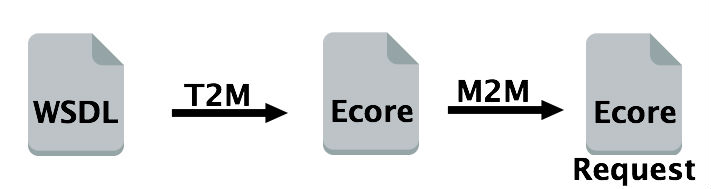
\includegraphics [scale=0.50]{imagenes/Transformacion_Wsdl_Ecore_Request.jpg}
	\end{center}
	\caption{Transformación Wsdl Ecore Request}
	\label{fig:Transformación Wsdl Ecore Request}
\end{figure} 

\begin{figure}[!h] 
	\begin{center}
		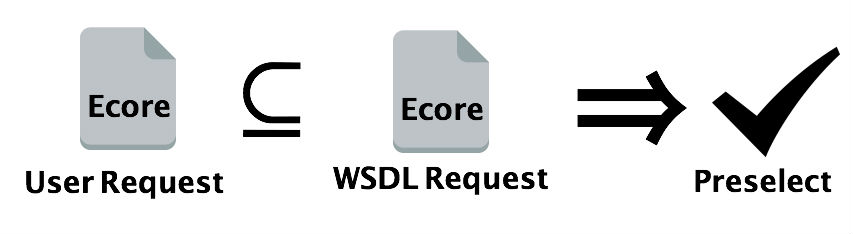
\includegraphics [scale=0.45]{imagenes/Comparacion_Ecore_Wsdl.jpg}
	\end{center}
	\caption{Comparación Ecore Wsdl - Ecore Request}
	\label{fig:Comparación Ecore Wsdl - Ecore Request}
\end{figure} 

\section{Modelos del solicitante y los proveedores de WS's}
\label{Modelos del solicitante y los proveedores de WS's}

Para la transformación de modelos, se debió utilizar dos modelos Ecore, uno que representa la solicitud del cliente, y el segundo representa un WS con formato WSDL.

\subsection{Modelo de solicitud de usuario}
\label{Modelo de solicitud de usuario}

Este modelo ecore se utiliza para representar una petición  de un cliente. La representación en diagrama de UML se realiza mediante el plugin Ecore Diagram Editor SDK\\

Un RequestModel tendrá asociado o no, uno o varios métodos, cada método deberá tener un nombre y posiblemente una descripción de lo que hace el método, el sistema buscará precandidatos en base al nombre del método. El método contendrá parámetros de entrada y salida, el cliente solo tendrá acceso a los parámetros de entrada. Cada parámetro deberá tener un tipo predefinido de Java y un nombre. (Ver figura \ref{fig:Diagrama UML de RequestModel})\\

Para obtener este modelo, se realiza una transformación T2M (ver código \ref{code:Transformación T2M RequestModel}), en donde se carga y genera un modelo RequestModel con los datos obtenidos desde una interfaz gráfica en la cual el usuario carga los requerimientos que desea.\\

\lstinputlisting[language=Java, firstline=103, lastline=161, caption={Transformación T2M RequestModel},label={code:Transformación T2M RequestModel}]{../QVTWSInvoker/src/tesis/controllers/InvokerController.java}





\begin{figure}[!h] 
	\begin{center}
		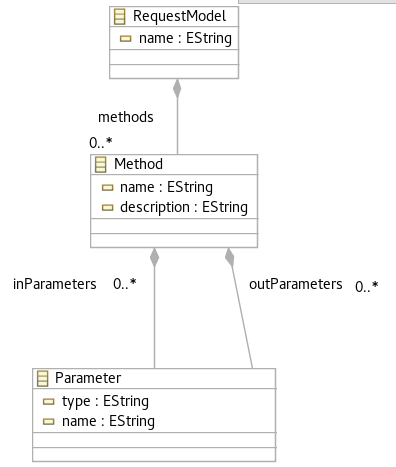
\includegraphics [scale=0.45]{imagenes/Diagrama_UML_RequestModel.png}
	\end{center}
	\caption{Diagrama UML de RequestModel}
	\label{fig:Diagrama UML de RequestModel}
\end{figure} 

Por otro lado un WS se representa mediante un modelo ecore WSDL, al cual se le ha agregando una descripción en las operaciones. \\

Para obtener un modelo ecore de este tipo, se realiza una transformación T2M, en donde el archivo con extensión .wsdl debe estar escrito en una versión de SOAP 1.1 o 1.2. 

\section{Estructura del proyecto de transformación}
\label{Estructura del proyecto de transformación}

El proyecto consiste de 3 módulos:
\begin{itemize}
	\item \textbf{T2MWsdl:} Este módulo realiza la transformación de texto a modelo de un wsdl
	\item \textbf{Comparsion:} Este módulo contiene la comparación de modelos, ambos modelos deben ser RequestModel.
	\item \textbf{Transformation:} Este módulo ejecuta en la transformación M2M de un wsdl, invocando la transformación QVTO definida.
\end{itemize}

Para la representación de los dos modelos ecore en Java,  se utilizó el plugin de eclipse EMF (Eclipse Modeling Framework SDK) que autogenera el código Java para la representación del mismo.\\
Esta representación en java consiste en 3 paquetes:

\begin{itemize}
	\item \textbf{utils:} Tiene clases auxiliares.
	\item \textbf{Impl:} Contiene la implementación de las interfaces.
	\item \textbf{Interface:} Comprende la representación de cada objeto del modelo ecore.
\end{itemize}

\section{Funcionamiento de la transformación}

El método consiste en 3 fases fundamentales, la primer etapa se encarga de la transformación de un wsdl en texto plano a un modelo ecore del mismo, la segunda etapa realiza la conversión M2M del modelo generado en la primer etapa a su respectiva representación en RequestModel, por último, la tercer etapa consiste en la comparación de 2 modelos RequestModel, el generado en la segunda etapa y la solicitud del usuario. Esta etapa deberá decidir si wsdl satisface la solicitud del usuario en base los criterios de comparación descritos al inicio del capítulo. \\

Ahora se explicará detalladamente cada etapa.\\

\textbf{Etapa 1: Transformación T2M wsdl}\\

Esta etapa realiza una transformación del wsdl en texto plano a una representación del mismo en ecore. Para ello, debemos conocer la ubicacion de algun WS, por ejemplo : \url{www.dominio\_del\_web\_service.com/servicio\_web.asmx?WSDL}\\

El sistema, con el soporte de la API soa\_model\_distribution, realiza un análisis gramatical del WS para hacer más eficiente su uso (ver código \ref{code:Transformación T2M RequestModel}), luego se procede a obtener los binding del WS que se encuentran definidos para trabajar con SOAP 1.1 y 1.2 y de cada binding se consiguen los PortType.

\lstinputlisting[language=Java, firstline=40, lastline=69,caption={Análisis gramatical del WS},label={code:Análisis gramatical del WS}]{../proyecto_eclipse/src/t2m/T2Mwsdl.java}

Luego a cada PortType, se le extraen las operaciones y se las analizan para obtener operaciones definidas en el modelo ecore.(ver código \ref{code:Extraccion de operaciones de PortType})

\lstinputlisting[language=Java, firstline=118, lastline=133,caption={Extracción de operaciones de PortType},label={code:Extraccion de operaciones de PortType}]{../proyecto_eclipse/src/t2m/T2Mwsdl.java}

Según la definición de un wsdl, cada operación consta de mensajes de entrada y mensajes de salida. Los mensajes pueden estar definidos con tipos simples, o utilizar tipos embebidos, a su vez, un tipo embebido puede contener otros tipos embebidos, por lo tanto se emplea la recursividad para “desenvolver” los parámetros y generar parámetros de tipos simples.(ver código \ref{code:Parser de messages} y \ref{code:Analisis y parser de tipos embebidos})

\lstinputlisting[language=Java, firstline=194, lastline=218,caption={Parser de messages},label={code:Parser de messages}]{../proyecto_eclipse/src/t2m/T2Mwsdl.java}

\lstinputlisting[language=Java, firstline=220, lastline=247,caption={Análisis y parser de tipos embebidos},label={code:Analisis y parser de tipos embebidos}]{../proyecto_eclipse/src/t2m/T2Mwsdl.java}

Al terminar todo el análisis, se obtiene el mismo wsdl pero cargado en un modelo ecore, el cual es exportado y almacenado en disco con una extensión .xmi para luego ser utilizado en la etapa 2.\\

\textbf{Etapa 2: Transformación qvto}\\

Esta etapa es la encargada de llevar a cabo la transformación qvto del modelo ecore wsdl en a un modelo ecore RequestModel. El sistema comienza tomando la ruta al archivo que se generó en la etapa anterior, y una ruta de salida, donde se almacenará el RequestModel.(ver código \ref{code:Invocación de la transformación qvto})

\lstinputlisting[language=Java, firstline=25, lastline=65,caption={Invocación de la transformación qvto},label={code:Invocación de la transformación qvto}]{../proyecto_eclipse/src/t2m/Transformation.java}

Este método, como se puede visualizar, invoca la transformación qvto almacenada en otra carpeta dentro del mismo proyecto. La transformación toma como archivo de entrada un modelo wsdl y retorna un modelo RequestModel.(ver código \ref{code:Perfiles y modelos de la transformación})


\lstinputlisting[ firstline=1, lastline=5,caption={Perfiles y modelos de la transformación},label={code:Perfiles y modelos de la transformación}]{../proyecto_eclipse/transforms/wsdlToRequest.qvto}

La transformación comienza buscando el objeto Definition en el wsdl, este es el que contiene toda la información necesaria para poder llevar adelante la transformación. Una vez obtenido la Definition, le aplica una transformación model2Request, obteniendo de esta forma el modelo RequestModel. (ver código \ref{code:Inicio de la transformación QVT})

\lstinputlisting[ firstline=7, lastline=20,caption={Inicio de la transformación QVT},label={code:Inicio de la transformación QVT}]{../proyecto_eclipse/transforms/wsdlToRequest.qvto}

Una vez dentro de Definition, el paso siguiente es,  asignar al RequestModel el nombre de Definition, y obtener los portType, que contiene la definición de los métodos, por lo tanto se le aplica una transformación portType2Methods, la cual retorna un conjunto de Methods pertenecientes al modelo RequestModel.(ver código \ref{code:Transformación PortType a Method})

\lstinputlisting[ firstline=22, lastline=36,caption={Transformación PortType a Method},label={code:Transformación PortType a Method}]{../proyecto_eclipse/transforms/wsdlToRequest.qvto}

De esta manera, se continúa transformando hasta llegar a la parte más “interna”, donde se encuentran los métodos.  Al finalizar la transformación, se consigue la representación del wsdl en RequestModel, el cual, únicamente, contiene la información necesaria, que son los métodos con sus respectivos parámetros de entrada y salida.\\

\textbf{Etapa 2: Comparación}\\

Una vez obtenido el/los wsdl representado/s en un modelo ecore RequestModel, y la petición del usuario, representado de la misma forma, se comparan para decidir si la petición está o no incluida en el wsdl, en caso de estarlo, se dirá que el wsdl resuelve la petición del usuario.\\
Esta comparación se realiza con comparaciones de modelos desde Java, tomando un wsdl y la petición del usuario y comparándolos por nombres de métodos, si los nombres coinciden, se continúa analizando la cantidad de parámetros de entrada que posee cada método, en caso de ser la misma, se analizan los tipos.  (ver código \ref{code:Transformación de un método})

\lstinputlisting[language=Java, firstline=15, lastline=62,caption={Transformación de un método},label={code:Transformación de un método}]{../proyecto_eclipse/src/t2m/Comparsion.java}

Para solucionar un error, se procedió a ordenar los parámetros de ambos modelos, de acuerdo al tipo, ya que la transformación qvto, es no determinista a la hora de aplicar una transformación, y puede desordenarlos.\\
Si los tipos son correctos, la comparación retorna una lista con los nombres de todos los métodos que satisfacen la petición del usuario.

\section{Análisis de la correspondencia entre los modelos generados}

Ahora, para decidir automáticamente si un WS ofrecido por un proveedor satisface la demanda del solicitante, es necesario comparar los ecore generados por dicho solicitante y proveedor. Se formaliza usando relaciones subecore. Si la precondición del solicitante es un subecore de la precondición del proveedor, entonces el proveedor provee toda la información necesaria para ejecutar el WS.\\
En la Figura \ref{fig:Ecores de Petición de usuario y WS 1} se puede observar que el modelo del WS 1 es un submodelo del modelo del solicitante.

\begin{figure}[!h] 
	\begin{center}
		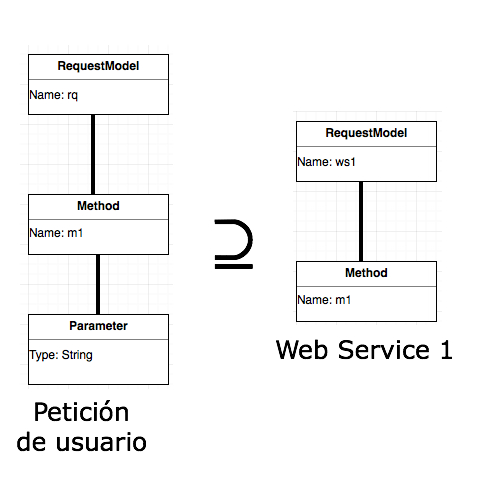
\includegraphics [scale=0.60]{imagenes/Ecores_de_Peticion_de_usuario_y_WS_1.jpg}
	\end{center}
	\caption{Ecores de Petición de usuario y WS 1}
	\label{fig:Ecores de Petición de usuario y WS 1}
\end{figure} 

\begin{figure}[!h] 
	\begin{center}
		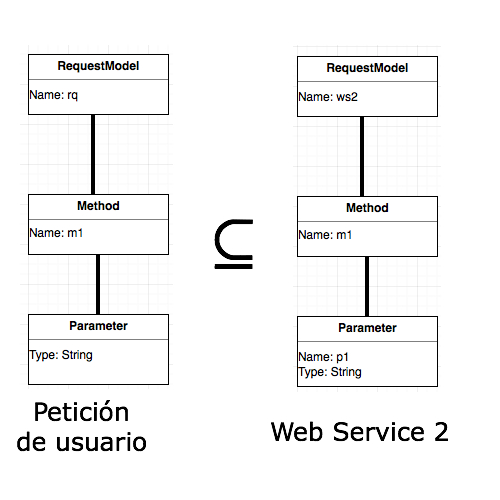
\includegraphics [scale=0.60]{imagenes/Ecores_de_Peticion_de_usuario_y_WS_2.jpg}
	\end{center}
	\caption{Ecores de Petición de usuario y WS 2}
	\label{fig:Ecores de Petición de usuario y WS 2}
\end{figure} 

Análogamente, en la Figura \ref{fig:Ecores de Petición de usuario y WS 2} se puede observar que la peticion de usuario es un submodelo del WS 2. Por lo tanto, el proveedor 2 ofrece un WS's que son compatibles con los requerimientos del solicitante. Entonces el proveedor 2 provee toda la información necesaria para ejecutar el WS.